%================================================================================
%       Safety Critical Systems Club - Data Safety Initiative Working Group
%================================================================================
%                       DDDD    SSSS  IIIII  W   W   GGGG
%                       D   D  S        I    W   W  G   
%                       D   D   SSS     I    W W W  G  GG
%                       D   D      S    I    WW WW  G   G
%                       DDDD   SSSS   IIIII  W   W   GGG
%================================================================================
%               Data Safety Guidance Document - LaTeX Source File
%================================================================================
%
% Description:
%   Appendix regarding Dark Data
%
%================================================================================
\section{Dark Data\index{Dark Data|textbf}\index{Data!Dark|see{Dark Data}} and Safety (Informative)} \label{bkm:darkdata}
%
%\dsiwgSectionQuote{Common sense tells us that the government's attempts to solve large problems more often create new ones. Common sense also tells us that a top-down, one-size-fits-all plan will not improve the workings of a nationwide health-care system that accounts for one-sixth of our economy}{Sarah Palin}
\dsiwgSectionQuote{\ldots we can be blind to missing data \ldots that can lead us to conclusions and actions that are mistaken, dangerous, or even disastrous.}{David Hand}

\subsection{Introduction}
This appendix outlines some of the safety implications arising from the issues identified by Prof. David Hand in his work on ``Dark Data'' presented in his book: ``Dark Data: Why What You Don't Know Matters'' \cite{citation:darkdata:hand} and website \cite{citation:darkdata:website}. Dark Data relates to data that is not available, but nevertheless is important, and indeed, in some cases, more important than the data that is available.

Unintentionally Donald Rumsfeld\index{Rumsfeld, Donald} popularised the concept of Dark Data with his famous speech:

\begin{quote}
\dsiwgTextIT{``…there are known knowns\index{Known Knowns}; there are things we know we know. We also know there are known unknowns\index{Known Unknowns}; that is to say we know there are some things we do not know. But there are also unknown unknowns\index{Unknown Unknowns}—the ones we don't know we don't know…''}
\end{quote}

\autoref{fig:lightanddark} neatly shows the dark varieties\index{Dark Data!Varieties} in grey:

\begin{figure}[htbp]
  \centering
  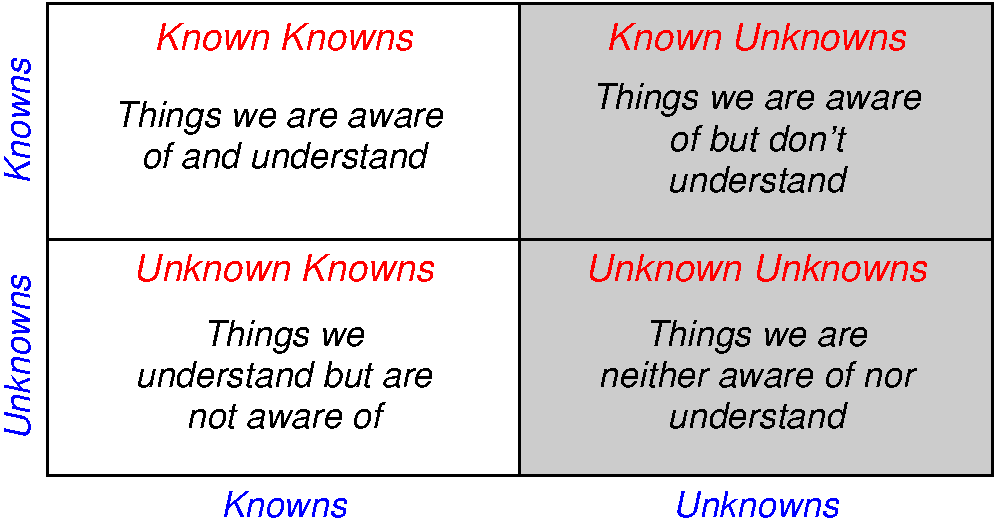
\includegraphics[width=\textwidth/2]{images/darkknowns.pdf}
  %\input{images/darkknowns.latex}
  \caption{Varieties of dark data\index{Dark Data!Varieties|textbf}}
  \label{fig:lightanddark}
\end{figure}\index{Unknown Knowns}

\subsection{Dark Data Example}
A meeting was held prior to the fatal Challenger disaster in January 1986, to decide whether the flight should go ahead due to the prevailing cold weather and concerns over the performance of O-ring seals at low temperatures. The decision to launch was made on the basis of the following data points that show the temperature at which previous O-ring problems had occurred.

\begin{figure}[htbp]
  \centering
  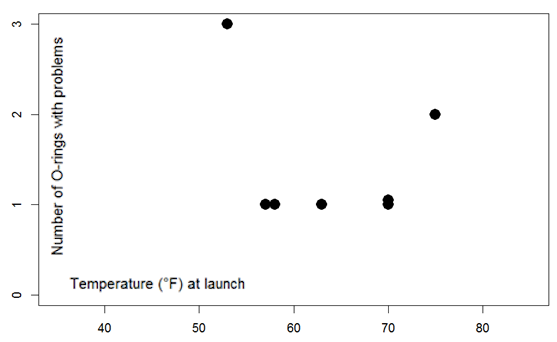
\includegraphics[width=\textwidth/2]{images/darkfailures}
  \caption{O-ring Failures by Temperature}
  \label{fig:o-ringfailures}
\end{figure}

On this basis, it was concluded that: 
``there is nothing irregular in the distribution of O-ring ‘distress’ over the spectrum of joint temperatures at launch between 53 degrees Fahrenheit and 75 degrees Fahrenheit.''
However, there was Dark Data in this dataset -- the data points that show the temperatures for successful launches when there were no O-ring problems were left out. These are shown as the red points in \autoref{fig:o-ringperformance}.

\begin{figure}[htbp]
  \centering
  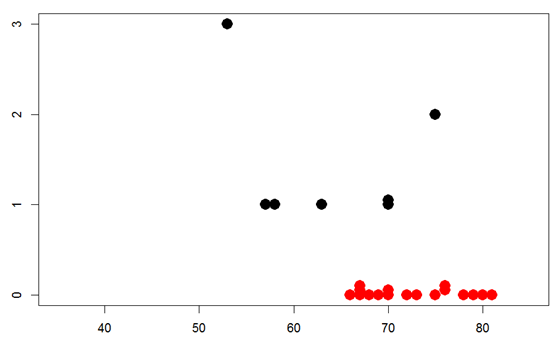
\includegraphics[width=\textwidth/2]{images/darkperformance}
  \caption{O-ring Performance by Temperature}
  \label{fig:o-ringperformance}
\end{figure}

When the Dark Data is included, there is an obvious correlation between temperature and O-ring failures and it is possible the decision to launch may have been different if this additional data had been presented.
\subsection{Dark Data Varieties\index{Dark Data!Varieties} and Safety Examples}
In his book, David introduces a taxonomy of 15 varieties of Dark Data. This section discuses each of these from a data safety perspective.

\subsubsection{Data We Know Are Missing: ``Known unknowns''}\index{Dark Data!Data We Know are Missing}\label{bkm:dark1}

This case is very common in safety justifications\index{Justification, Safety} where assurance information may be withheld for commercial reasons or does not exist, but we know, or are informed, that it isn’t available. Common examples include:
\begin{itemize}
  \item Assurance information for \gls{cots}\index{COTS} components is unavailable
  \item Information about legacy systems was never produced or is now lost
  \item ML training data restricted to a particular context of use
\end{itemize}
    If this is the case, it can be mitigated\index{Mitigation} in several ways, including use of warnings, training, restrictions of use, etc. Evidence can also be substituted with other more indirect assurance e.g.\ established organizational track-record in the sector, or audit reports.
    
\subsubsection{Data We Don’t Know Are Missing: ``Unknown unknowns''}\index{Dark Data!Data We Don't Know are Missing|textbf}\index{Unknown Unknowns}\label{bkm:dark2}
This is the most serious and far-reaching case. Occurrence is hopefully less common than case~\ref{bkm:dark1}, but it is important to acknowledge that it does happen. Some examples are:
\begin{itemize}
  \item The recent Covid-19 Track and Trace data loss (\autoref{bkm:incacc:covidexcel}), where the organization handling the data was unaware that rows were missing from a spreadsheet for some time is illustrated in \autoref {fig:darknewcases}
  \item Somebody knows a problem with a system but does not tell
  \item Machine learning training data\index{Machine Learning Data} missing edge / corner cases
  \item Key \index{Safety Requirement}safety requirements missed
  \item Change of use never anticipated
  \item Data loss which may be discovered after some period (or indeed never) 
  \item Test cases never thought of, so never created or executed
\end{itemize}

\begin{figure}[htbp]
  \centering
  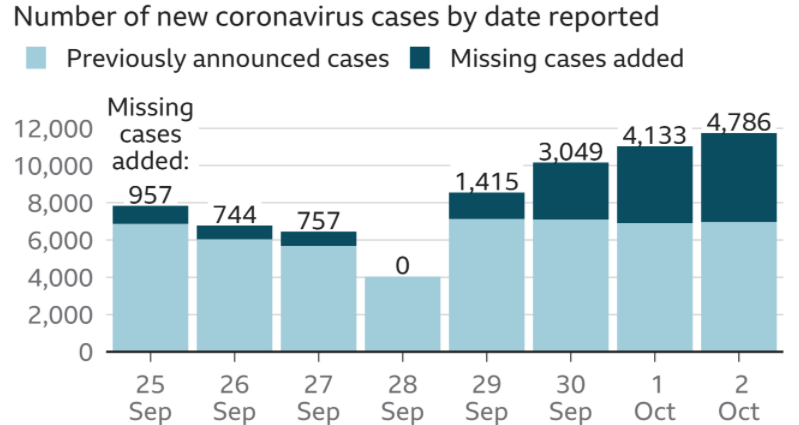
\includegraphics[width=\textwidth/2]{images/darknewcases}
  \caption{Covid-19 Track and Trace Data Loss}
  \label{fig:darknewcases}
\end{figure}

In many cases the loss may be discovered after some time, and it is incumbent on the organization involved to analyse the impact of the missing data over the time period, including subsequent decisions and actions. Its effects should not be underestimated. This case can fundamentally change the safety picture and is probably in the highest safety risk category.

Data that was missing can subsequently be found. The following options show possible approaches to handling this “rediscovered data”:
\begin{enumerate}[label=\color{dsiwgAccentColour}\roman*)]
  \item Apply the missing data
  \item Ignore the missing data 
  \item Mention that the data was missing but not take it into account, and 
  \item Perform an impact analysis on the missing data and then act according to the results
\end{enumerate}

\subsubsection{Choosing Just Some Cases}\index{Dark Data!Choosing Just Some Cases}\label{bkm:dark3}
This is where something or somebody has been selective. Examples might be:
\begin{itemize}
\item Selection of test runs that succeeded (ignoring failed runs and their diagnostics) 
  \item Selective sampling from sensors, or where the sampling intervals are chosen badly
  \item Incorrect filtering of the data, leaving out more cases than intended
  \item Using data from completed forms, finished tasks or only including data which,
    intentionally or not, meets some criteria which excludes the important data.
    This can lead to "Survivorship Bias",
    [Wikipedia ref:
      \href{https://en.wikipedia.org/wiki/Survivorship\_bias}
           {https://en.wikipedia.org/wiki/Survivorship\_bias}]
    of which the following article has a good example from WW2 aircraft where examining the bullet
    holes on aircraft returning from missions could have led to the wrong conclusion:
    \href{https://www.dgsiegel.net/talks/the-bullet-hole-misconception}
         {https://www.dgsiegel.net/talks/the-bullet-hole-misconception}
\end{itemize}
Note that with complex or informal criteria the effects could be as case~\ref{bkm:dark2}, i.e.\ you don’t know what has been left out.

Mitigations\index{Mitigation} include use of peer review, independent teams, and audits. It is important to ask questions and challenge the data selected to be sure it can be justified.
\subsubsection{Self-Selection}\index{Dark Data!Self-selection}\label{bkm:dark4}
This is considered to be similar to case~\ref{bkm:dark3}, but could be even more informal or ambiguous. Again mitigations\index{Mitigation} include: use of peer review, independent teams, and audits.

\subsubsection{Missing What Matters}\index{Dark Data!Missing What Matters|textbf}\label{bkm:dark5}
This was considered similar to case~\ref{bkm:dark2} in impact terms, and might well be considered the “Elephant in the Room”. Examples might be:
\begin{itemize}
\item Measuring the wrong things, e.g.\ poor safety metrics / indicators
  \item Too much data to deal with or analyse, so some is ignored
  \item Too much filtering or processing, so losing information along the way
  \item Being too close to the data, i.e.\ the “wood for the trees”. This is when the detail masks the overall issue with data, e.g.\ a slow trend or bias masked by peaks.
\end{itemize}

Mitigations\index{Mitigation} include independence as~\ref{bkm:dark3} and~\ref{bkm:dark4} but also “taking a step back” to look at the bigger picture.
\subsubsection{Data Which Might Have Been}\index{Dark Data!Data Which Might Have Been}\label{bkm:dark6}
This is where it is impossible to obtain the relevant data as a consequence of how the system/scenario is constructed. This was considered an interesting and important case.

This could for example, be due to an inappropriate system architecture e.g.\ single data channel when a multiple channel approach should have been used, such as in the \index{Boeing 737}Boeing 737 MAX~8 accidents (see section H.2). It is therefore important that Mitigations\index{Mitigation} are in place at design time, as they are often very difficult to retro-fit.

Mitigations\index{Mitigation} include assessing the data collection opportunities gained or lost from the design or architectural approach -- at design time.

\subsubsection{Changes with Time}\index{Dark Data!Changes With Time}\label{bkm:dark7}
This is a common problem in a safety context. Data in safety systems often becomes obsolete or out of date and may still be mistakenly used. Some examples are:
\begin{itemize}
\item System configuration data not kept up to date as software\index{Software Changes} or hardware changes
  \item Medical drug interaction databases
  \item Software patches requiring updates to configuration or system data, which is not always done
\end{itemize}

Mitigations\index{Mitigation} include keeping critical data up to date and regularly refreshed, and knowing how old the data is in the first place.

\subsubsection{Definitions of Data}\index{Dark Data!Definitions of Data}\label{bkm:dark8}
This was considered a common case for systems with databases or those exchanging data with external systems, e.g.
\begin{itemize}
\item Taxonomies e.g.\ in machine learning categorisation schemes
  \item Data schemas in medical record systems 
  \item Interface specifications\index{Interface!Specification} and data definitions\index{Data!Definition}, which often evolve over time. These can render old data obsolete / subject to misinterpretation, and often needing migration/translation or re-interpretation.
\end{itemize}

Mitigations\index{Mitigation} include keeping a list of known changes / incompatibilities and documenting the changes or fixes that have to be applied to make the data usable or consistent.

\subsubsection{Summaries of Data}\index{Dark Data!Summaries of Data}\label{bkm:dark9}
This is often seen in data about safety systems and projects:
\begin{itemize}
\item Safety metrics or indicators where data is aggregated to create a composite value
  \item Data fusion across multiple sensors
Summaries can be misleading or cause “boundary reactions”, e.g. Red-Amber boundary.
\end{itemize}

Mitigations\index{Mitigation} include thinking about what missing data could cause (i.e.\ performing sensitivity analysis) -- for instance, what decisions might be made erroneously due to certain data values being omitted, late or slightly perturbed.

\subsubsection{Measurement Error and Uncertainty}\index{Dark Data!Measurement Error and Uncertainty}\label{bkm:dark10}
Sensors can degrade and fail over time, especially in harsh environments such as automotive, marine or aviation:
\begin{itemize}
\item Sensors may feed faulty or biased data into systems
  \item Sampling techniques can cause some artefacts in themselves
  \item Interval polling interval can lead to misleading readings
  \item Data fusion can be impacted if multiple sensor values are combined
\end{itemize}

Hence sensors need to be regularly maintained and calibrated or replaced, and their interfaces\index{Interface!Sensor} need to be able to detect any problems and report faults. 

\subsubsection{Feedback and Gaming}\index{Dark Data!Feedback and Gaming}\label{bkm:dark11}
This can often happen in safety justifications\index{Justification!Safety} or test case production:
\begin{itemize}
\item Early production of a safety argument could lead to only those artefacts that support the claim being generated, e.g.\ requirements-based testing vs.\ stress testing
  \item Confirmation bias in safety justifications\index{Justification, Safety} and can cause over-optimism
\end{itemize}

Mitigations\index{Mitigation} include the use of dialectic argument approaches (where both positive and negative cases can be considered). It is also useful to get a second opinion, independent review or a ‘fresh pair of eyes’ to check the justification.

\subsubsection{Information Asymmetry}\index{Dark Data!Information Assymetry}\label{bkm:dark12}
This is common where there are multiple stores or sources of the same data:
\begin{itemize}
\item Multiple / backup databases where they are not kept in sync
  \item Image recognition systems that learn, but fail to share data
  \item Issues of divergence of data across multiple sources.
\end{itemize}

Comparisons, reviews and data audits may help in these cases. In general the issue of divergence across multiple data sources needs to be recognized and addressed in the most appropriate technical, and ideally automated, way.

\subsubsection{Intentionally Darkened Data}\index{Dark Data!Intentionally Darkened Data}\label{bkm:dark13}
This can and does happen, e.g.
\begin{itemize}
\item Defence, security and government sectors where data is purposefully hidden or destroyed
  \item Records intentionally deleted after an accident to cover up what really happened
\end{itemize}

This can be mitigated\index{Mitigation} using appropriate technical measures (e.g.\ blockchain, digital signatures, off-site backups), and also robust procedures with oversight.

\subsubsection{Fabricated and Synthetic Data}\index{Dark Data!Fabricated and Synthetic Data}\label{bkm:dark14}
Fabrication (i.e.\ making up the data) is surprisingly common, e.g.\ in medical, policing and maritime sectors. Sometimes it is created with the best of intentions as it was not produced or collected at the right time and is now required (e.g.\ for an audit), but sometimes it is created to mask a problem. Synthetic data is often used where there are difficulties in producing enough real data with the right characteristics:
\begin{itemize}
\item Data is retrospectively entered / patched to make a “clean” record
  \item Synthetic autonomous vehicle training databases can have issues with artificial data if not realistic
\end{itemize}

Possible mitigations\index{Mitigation} include comparisons with current real-world data and checking with historical data.

\subsubsection{Extrapolating Beyond Your Data}\index{Dark Data!Extrapolating Beyond Your Data}\label{bkm:dark15}
Systems, especially machine learning systems (see Appendix J) have to cope with values outside of their training data\index{Machine Learning Data}, but the outcomes may be unexpected:
\begin{itemize}
\item Bizarre results from recognition / detection systems may result
\end{itemize}

Mitigations\index{Mitigation} include use of machine learning training data\index{Machine Learning Data} containing edge/corner cases, boundary cases, and testing well beyond normal or acceptable ranges to give insight into the system degradation behaviour.

\subsection{Summary}
Dark Data is a very useful way of thinking about problems and solutions. It is important to always think of the bigger picture, considering what information is not known:

\begin{itemize}
  \item What might have been left out, intentionally or otherwise?
  \item What might be missing due to the way things are done (or the way those things are being executed)?
  \item Could missing items cause any safety problems?
  \item What is outside of the defined operational domain?
  \item Can you present your results / outputs in a way that shows the dark data?
\end{itemize}

\subsection{Further Reading}
A number of resources are available for further information on how Dark Data relates to data safety:
\begin{itemize}
\item The October 2020 edition of the SCSC Newsletter \cite{citation:SCSC160} contains articles both by David Hand and on Dark Data Safety.
  \item A presentation on Dark Data given by David Hand to the \gls{dsiwg} \cite{citation:darkdata:presentation1};
  \item A presentation by Mike Parsons given at the University of York \cite{citation:darkdata:presentation2}.
\end{itemize}
